\documentclass[]{IEEEtran}

\title{Modellazione e Sintesi di un Moltiplicatore Floating-point Single Precision}
\author{Enrico Sgarbanti - VR446095}

\usepackage{graphicx}
\usepackage[italian]{babel}
\usepackage[utf8]{inputenc}

\begin{document}
\maketitle

\begin{abstract}
Il progetto ha 3 diversi obiettivi:
\begin{itemize}
\item Sviluppare in VHDL, Verilog e SystemC un componente che esegua due moltiplicazioni in virgola mobile a precisione singola
\item Sintetizzare i componenti scritti in VHDL e Verilog
\item Eseguire High-Level-Synthesis del moltiplicatore a precisione singola
\end{itemize}
\end{abstract}


\section{Introduzione}
Il sistema è composto da un modulo top-level chiamato ``double\textunderscore multiplier'' il quale esegue la moltiplicazione di due operandi dati in input nello stesso ciclo di clock in cui ready viene posto a 1, e i due opereandi passati al ciclo di clock successivo
\\

Nell'introduzione viene descritto in maniera astratta quello che poi viene dettagliato nel seguito del report. Una buona scaletta per l'introduzione può essere la seguente:
\begin{itemize}
\item Descrizione ad alto livello delle principali caratteristiche del sistema che si vuole modellare.
\item Descrizione delle motivazioni principali per l'utilizzo delle tecnologie descritte nel corso. Qual è il problema che si vuole risolvere?
\item Descrizione dei passi utilizzati per arrivare all'implementazione finale. Descrivere la motivazione di ciascun passo. La descrizione dei passi dovrebbe formare la descrizione del flusso di lavoro svolto per completare l'assignment.
\item Rapidissima descrizione dei risultati principali.
\end{itemize}

L'introduzione non dovrebbe andare oltre la metà della seconda colonna (nel caso a due colonne), o la prima pagina (nel caso a colonna singola): bisogna cercare di essere concisi (e chiari). Alla fine, l'introduzione è solo ``chiacchiere'': deve semplicemente rendere chiari quali sono gli obiettivi del lavoro (\emph{e nel caso del corso, deve far capire a me che avete gli obiettivi chiari in testa}). Consiglio: l'introduzione (e spesso l'abstract) è l'ultima parte che viene completata.

\section{Background}

- descrivere cos'è un floating-point
- descrivere la moltiplicazione
- arrotondamento numero binario

Il background dovrebbe contenere una descrizione, abbastanza breve, dei concetti principali che vengono utilizzati nel lavoro. Ad esempio, può contenere una breve descrizione delle caratteristiche principali degli HDL , e delle sue estensioni. Una colonna dovrebbe bastare.

In questa sessione saranno citati anche lavori dello stato dell'arte. Ad esempio, si può usare~\cite{SystemC} per citare SystemC. \textbf{I riferimenti bibliografici vanno inseriti ogni volta in cui si va a citare qualcosa contenuto in un documento.}

Questa sessione non deve ripetere quanto detto a lezione, ma dare un overview dei concetti principali utilizzati durante lo svolgimento dell'elaborato.


\section{Metodologia applicata}
Attuando un approccio bottom-up, prima si definiscono i componenti principali cioè il {\it moltiplicatore} e il {\it doppio moltiplicatore}, descrivoli con EFSM. Dopodichè si passa all'implementazione a livello RTL in vhdl e verilog di queste e alla creazione di un piccolo testbench. A questo punto si traduce il tutto in systemC dove con la potenza del C++ si crea un testbench più complesso. Infine si procede alla sintesi e alla sintesi ad alto livello per poi confrontare i vari risultati.

\subsection{Modellazione della EFSM del moltiplicatore}
I segnali utilizzati sono:
\begin{itemize}
\item {\it\bf rst:} (1 bit) per riportare il sistema allo stato iniziale .
\item {\it\bf ready:} (1 bit) per permettere al sistema di uscire dallo stato iniziale .
\item {\it\bf norm\textunderscore again:} (1 bit) per indicare se fare un'altra normalizzazione del numero intermedio.
\item {\it\bf res\textunderscore type:} (2 bit) per indicare se il risultato vale 0, NAN o \(\infty\) e quindi andare direttamente allo stato finale oppure se è un numero (il caso denormalizzato viene gestito come se fosse normalizzato) e quindi proseguire nell'elaborazione.
\end{itemize}

Sono inoltre necessari 14 stati:
\begin{itemize}
\item {\it\bf ST\textunderscore START:} in cui si pone {\it done} e {\it norm\textunderscore again} uguali a 0 e si ottengono le informazioni di segno, esponente e mantissa dei due operandi. In esso si rimane finchè {\it ready} vale 0 altrimensi si passa a {\it ST\textunderscore EVAL1}.
\item {\it\bf ST\textunderscore EVAL1:} e {\it ST\textunderscore EVAL2} in cui viene valutato il tipo dei due operandi fra {\it T\textunderscore ZER, T\textunderscore INF, T\textunderscore NAN e T\textunderscore NUM}
\item {\it\bf ST\textunderscore EVAL3:} in cui si ricava il tipo del risultato in base al tipo degli operandi.
\item {\it\bf ST\textunderscore CHECK1:} dove si passa a {\it ST\textunderscore FINISH} se {\it res\textunderscore type} è diverso da {\it T\textunderscore NUM}.
\item {\it\bf ST\textunderscore ELAB:} in cui si sommano i due esponenti e si sottrae 127 perchè entrambi, per lo standard, sono incrementati di 127 (\((esp+127) = (esp1+127)+(esp127) - 127\)). Per compiere la somma è necessario usare una variabile ``esp\textunderscore tmp'' 10 bit altrimenti si andrebbe in overflow per valori invece leciti che ritornerebbero validi dopo la sottrazione di 127. Inoltre viene eseguita anche la moltiplicazione delle due mantisse, che essendo a 23 bit più un bit che vale sempre 1, necessita di una variabile ``mant\textunderscore tmp'' di 48 bit 
\item {\it\bf ST\textunderscore UNDERF:} in cui si verifica se l'esponente del risultato è in uno stato di underflow, ovvero guardando se il bit {\it esp\textunderscore tmp[9]}, che nel complemento a 2 indica il segno, è 1. Infatti i valori disponibili per l'esponente vanno da 0 a 255.
\item {\it\bf ST\textunderscore CHECK2} dove si passa a {\it ST\textunderscore FINISH} se {\it res\textunderscore type} è diverso da {\it T\textunderscore NUM}, perchè diventato {\it T\textunderscore ZER} per l'underflow.
\item {\it\bf ST\textunderscore NORM1:} in cui si compie la normalizzazione della mantissa che deve sempre essere della forma {\it 1.valori}. Essendo la virgola posta tra il 46esimo bit e il 45esimo, si verificano due casi: Se il 47esimo bit vale 1 bisogna incrementare l'esponente, altrimenti il valore è già corretto, ma viene effettuato uno shift a sinistra per trattare allo stesso modo i due casi durante l'arrotondamento.
\item {\it\bf ST\textunderscore ROUND:} in cui si effettua l'eventuale arrotondamento dovuto al fatto che il valore della mantissa è attualmente a 48 bit, ma bisogna portarlo a 24 bit. L'arrotondamento è fatto per eccesso, quindi si incrementerà {\it mant\textunderscore tmp[47:24]} solo se {\it mant\textunderscore tmp[23:00]} sarà \( \geq \) a ``01..1''. L'arrotondamento effettivò verrà fatto nello stato {\it ST\textunderscore NORM2}, qui ci si limita a porre {\it norm\textunderscore again} uguale a 1 per poterci andare.
\item {\it\bf ST\textunderscore CHECK3:} dove si passa a {\it ST\textunderscore NORM2} se {\it norm\textunderscore again} è uguale a 1 altrimenti a {\it ST\textunderscore OVERF} per il controllo di eventuali overflow
\item {\it\bf ST\textunderscore NORM2:} in cui si effettua il vero arrotondamento della mantassina. Bisogna tenere conto del caso in cui sia della forma ``1..1'' e che quindi con l'incremento vada a ``0..0'' e  venga incrementato l'esponente.
\item {\it\bf ST\textunderscore OVERF:} in cui si verifica se l'esponente del risultato è in uno stato di overflow, ovvero guardando se il bit {\it esp\textunderscore tmp[8]} vale 1 ovvero se corrisponde ad un valore maggiore di 255.
\item {\it\bf ST\textunderscore FINISH:} in cui si pone {\it done} uguale 1, si ricava {\it res[31]}, ovvero il segno del risultato facendo lo XOR fra i segni degli operandi, e in base al valore di {\it res\textunderscore type} si ottiene il resto. Dopodichè si torna allo stato inziale
\end{itemize}


\subsection{Modellazione della EFSM del doppio moltiplicatore}
I segnali utilizzati sono:
\begin{itemize}
\item {\it\bf rst:} (1 bit) per riportare il sistema allo stato iniziale .
\item {\it\bf ready:} (1 bit) per permettere al sistema di uscire dallo stato iniziale .
\item {\it\bf done1:} (1 bit) che indica quando il valore attuale di ``res1'' è il risultato della moltiplicazione.
\item {\it\bf done2:} (1 bit) che indica quando il valore attuale di ``res2'' è il risultato della moltiplicazione.
\end{itemize}

Sono inoltre necessari 8 stati:

\begin{itemize}
\item {\it\bf ST\textunderscore START:} in cui si pone {\it done}, {\it ready1} e {\it ready2}uguali a 0 e si inizializzano {\it op1_tmp1} e {\it op2_tmp1} rispettivamenete con i valori di {\it op1} e {\it op2} i quali serviranno per il primo moltiplicatore. In esso si rimane finchè {\it ready} vale 0 altrimensi si passa a {\it ST\textunderscore RUN1}.
\item {\it\bf ST\textunderscore RUN1:} in cui si pone {\it ready1} uguale a 1, attivando quindi il primo moltiplicatore, e si inizializzano {\it op1_tmp2} e {\it op2_tmp2} rispettivamenete con i valori di {\it op1} e {\it op2} i quali serviranno per il secondo moltiplicatore.
\item {\it\bf ST\textunderscore RUN2:} in cui si pone {\it ready1} uguale a 0 e {\it ready2} uguale a 1, attivando quindi il secondo moltiplicatore
\item {\it\bf ST\textunderscore WAIT:} in cui si pone {\it ready2} uguale a 0 e si aspetta che {\it done1} o {\it done2} diventino 1.
\item {\it\bf ST\textunderscore WAIT1:} si arriva in questo stato se {\it done2} vale 1, cioè se il secondo moltiplicatore ha finito e si resta qui finchè non finisce anche il primo.
\item {\it\bf ST\textunderscore WAIT2:} si arriva in questo stato se {\it done1} vale 1, cioè se il primo moltiplicatore ha finito e si resta qui finchè non finisce anche il secondo.
\item {\it\bf ST\textunderscore RET1:} si arriva in questo stato quando entrambi i moltiplicatore hanno finito. Qui si pone {\it done} uguale a 1 e {\it res} uguale al risultato del primo moltiplicatore cioè {\it res1}.
\item {\it\bf ST\textunderscore RET2:} ora si pone {\it res} uguale al risultato del secondo moltiplicatore cioè {\it res2} e si ritorna allo stato iniziale.
\end{itemize}


\subsection{Implementazione RTL con Verilog e VHDL}
Si creano i seguenti files:
\begin{itemize}
\item {\it\bf verilog_multiplier:} implementazione verilog del moltiplicatore (sintetizzabile)
\item {\it\bf vhdl_multiplier:} implementazione vhdl del moltiplicatore (sintetizzabile)
\item {\it\bf double_multiplier:} implementazione verilog del doppio moltiplicatore (sintetizzabile)
\item {\it\bf testbench:} implementazione verilog di un testbench da usare solo in simulazione
\end{itemize}


\subsection{Implementazione RTL con SystemC}
Si creano i seguenti files e directory:
\begin{itemize}
\item {\it\bf Makefile:} tool per la compilazione automatica del progetto. Richiede che la variabile d'ambiente SYSTEMC_HOME contenga il path alla libreria di SystemC.
\item {\it\bf bin:} directory che contiene l'eseguibile {\it double_multiplier_RLT.x} (generato dopo la compilazione) e {\it wave.vcd} (generato dopo l'esecuzione dell'eseguibile).
\item {\it\bf obj:} directory che contiene i files oggetto (generati dopo la compilazione)
\item {\it\bf include:} directory che contiene gli headers {\it double_multiplier_RTL.hh}, {\it multiplier_RTL.hh}, {\it testbench_RTL.hh}.
\item {\it\bf testbench:} directory che contiene i files sorgenti {\it double_multiplier_RTL.cc}, {\it multiplier_RTL.cc}, {\it testbench_RTL.cc} e {\it main_RTL.cc}.
\end{itemize}


In questa sezione viene descritto tutto il procedimento, ed è dunque la sezione più importante del report. Va descritto passo passo quello che avete fatto, facendo capire ``esattamente'' cosa è stato fatto.

Questa sezione può essere divisa in sottosezioni. Le informazioni riportate nella lista seguente dovrebbero essere identificabili nel testo del report (\textbf{anche in ordine diverso}):
\begin{itemize}
\item Definizione dell-architettura del programma
\item Descrizione del componente di HW digitale.
\item Processo di ``sintesi'' verso RTL. Definizione dei sottocomponenti del componente HW, e della sua struttura. Definizione dell'interfaccia RTL, definizione della Macchina a Stati Finiti Estesa (EFSM) del componente e dei sottocomponenti. Realizzazione del componente HW utilizzando i processi in diversi stili a livello RTL. \`E inoltre possibile discutere la scelta dei tipi di dato.
%\item Descrizione della realizzazione della parte rappresentante SW Embedded, e descritta in TLM.
%\item Descrizione della realizzazione della parte a tempo continuo. Spiegazione delle scelte progettuali fatte per gli stili di modellazione utilizzati.
\item Descrizione dei meccanismi di comunicazione tra le diverse parti del sistema.
\end{itemize}

\textbf{In questa sezione deve essere riportato (brevemente) anche l'organizzazione dell'implementazione consegnata assieme al report.}

\section{Risultati}

Qua vanno ``messi i numeri''. Questa sezione dovrebbe contenere i risultati della simulazione. La simulazione mostra che il sistema funziona correttamente? Com'è stato provato? Che tipo di testbench sono stati utilizzati? Com'è stato scomposto il sistema per verificarne la correttezza?

Per quanto riguarda le performance:
\begin{itemize}
\item cosa si può dire in merito alla latenza?
\item Qual è la frequenza massima del design? 
\item Qual è l'area occupata dal design? 
\end{itemize}

Questa sezione può contenere anche riflessioni personali sui risultati ottenuti. Importante: tutte le affermazioni devono essere supportate da numeri\footnote{Richard Feynman on Scientific Method (1964) -\\ https://www.youtube.com/watch?v=OL6-x0modwY}.

\section{Conclusioni}
Le conclusioni dovrebbero riassumere in poche righe  tutto ciò che è stato fatto. Un paio di righe descrivono i risultati osservati, in modo da introdurre poi la conclusione ``vera e propria''. Nel caso del corso, la ``lezione da portare a casa'' sarà quello che si è imparato svolgendo l'elaborato.


\bibliographystyle{IEEEtran}
\bibliography{biblio}

\appendix
Se non avete abbastanza spazio, potete inserire le figure delle EFSM in una  pagina extra, appendice. Un esempio di come potete fare solo le Figure~\ref{fig:grande}, \ref{fig:piccola1}, \ref{fig:piccola2}.


\begin{figure*}[bt]
\centering
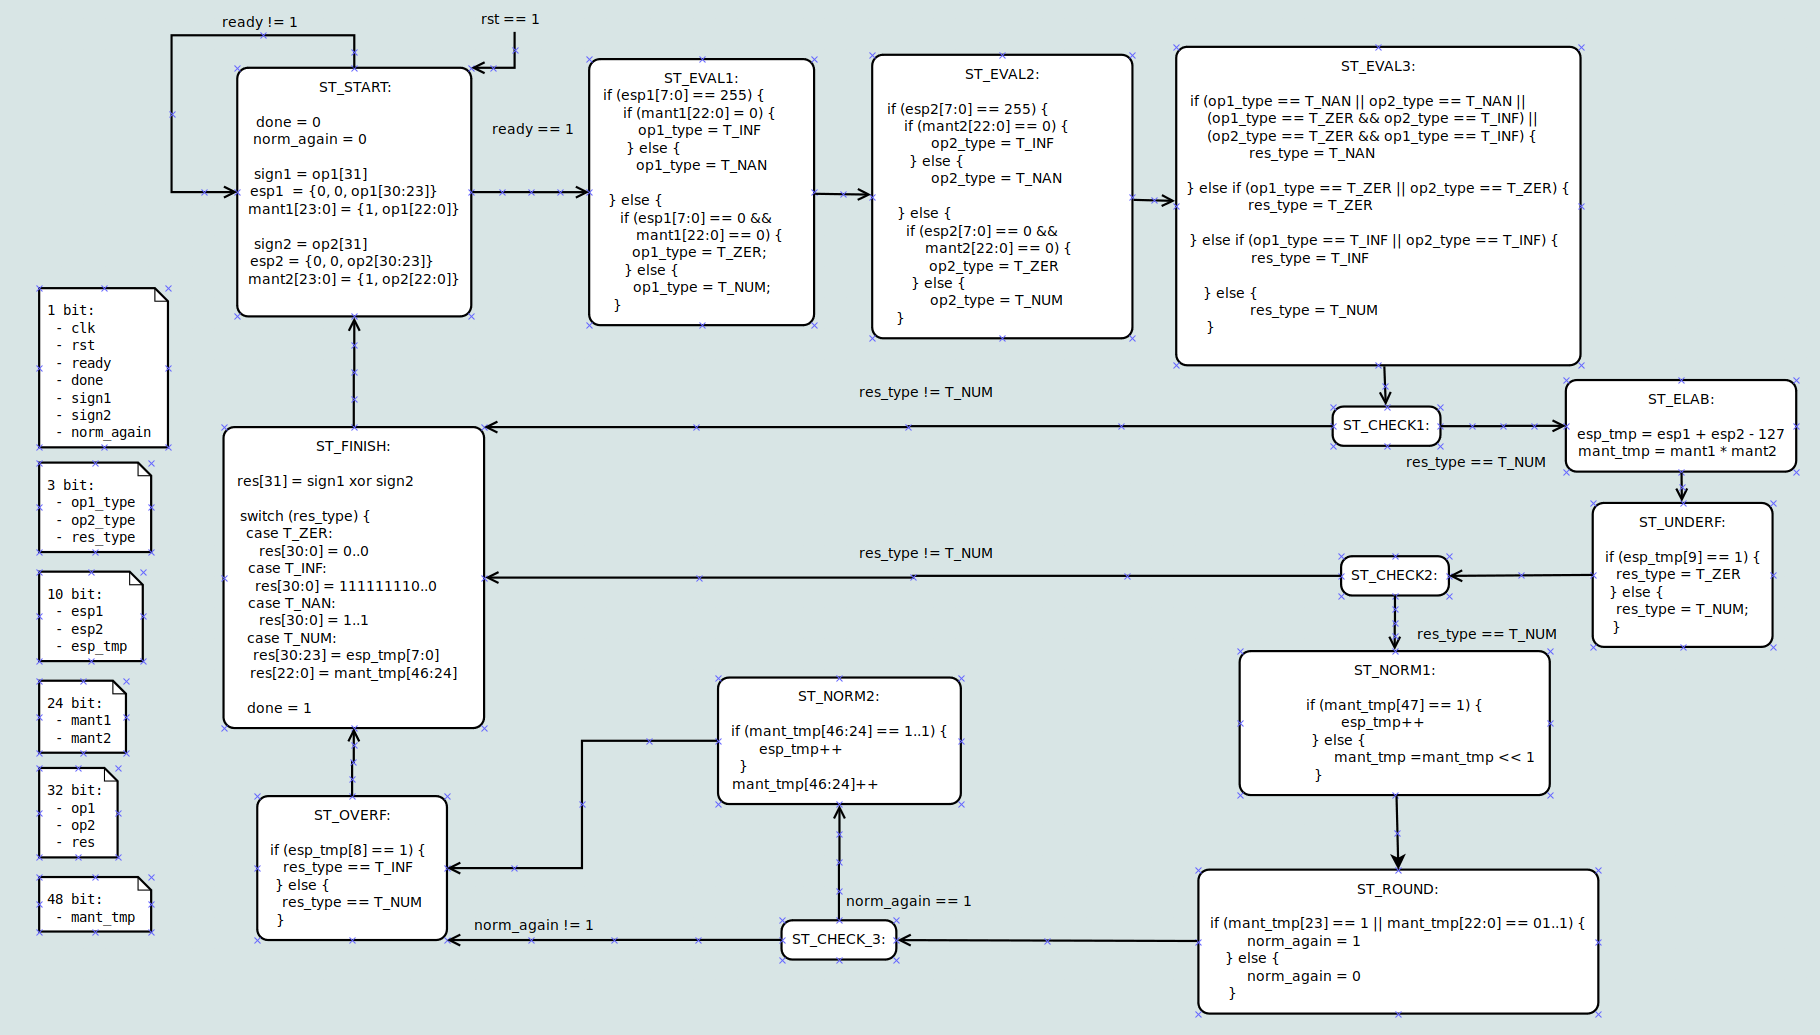
\includegraphics[width=\textwidth]{figures/EFSM-multiplier}
\caption{Figura in formato grande.}
\label{fig:grande}
\end{figure*}

\begin{figure}[bt]
	\centering
	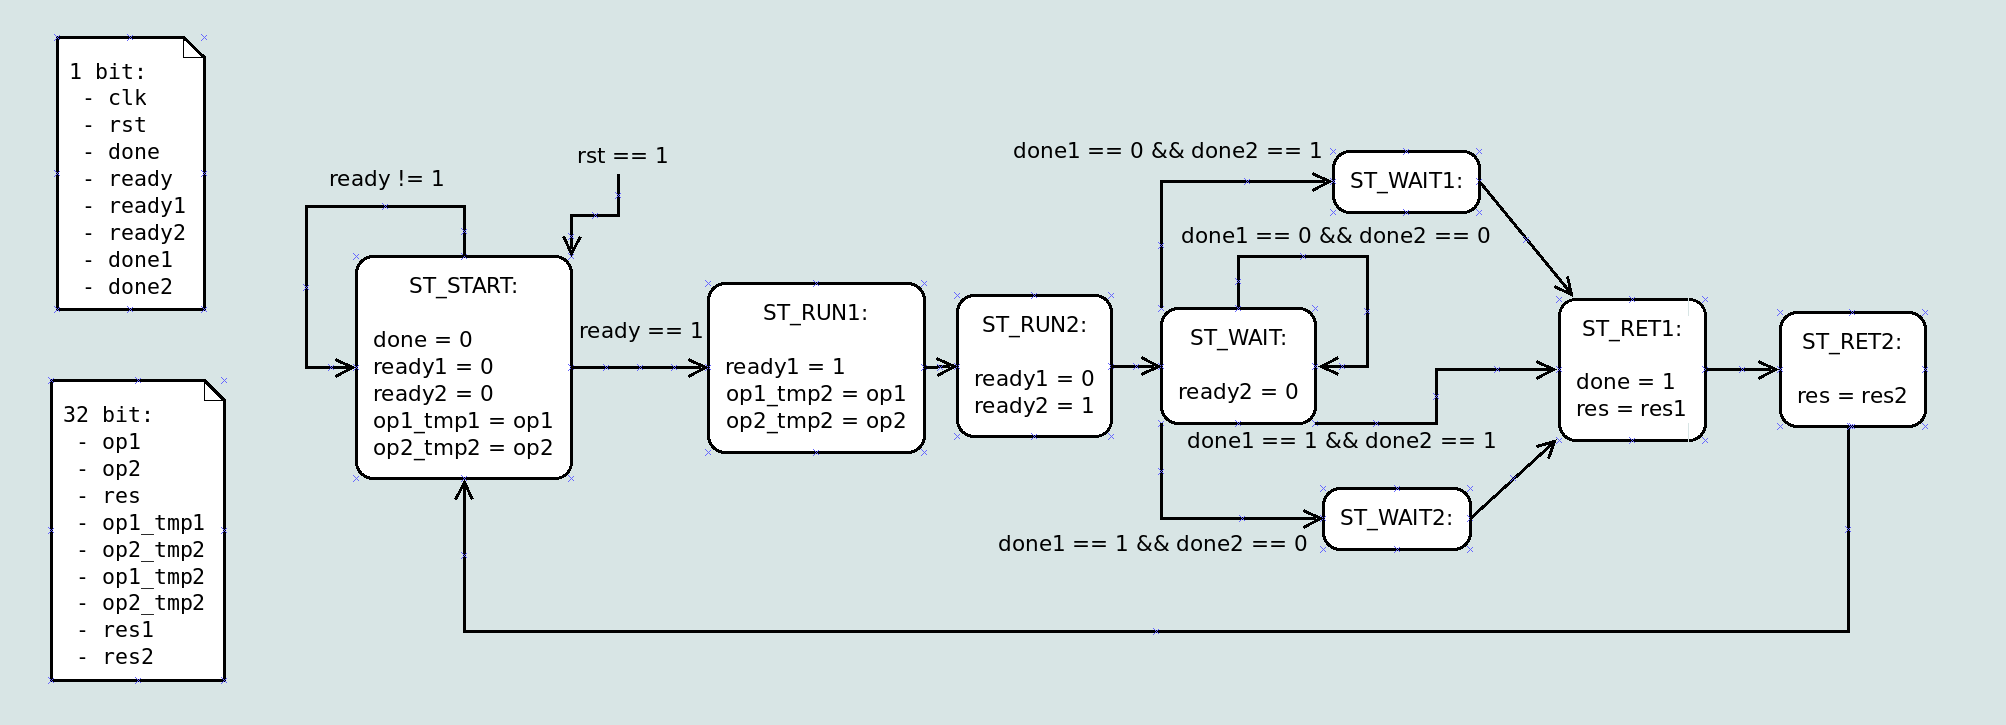
\includegraphics[width=\columnwidth]{figures/EFSM-top_level}
	\caption{Figura in formato piccolo, 1.}
	\label{fig:piccola1}
\end{figure}

\begin{figure}[bt]
	\centering
	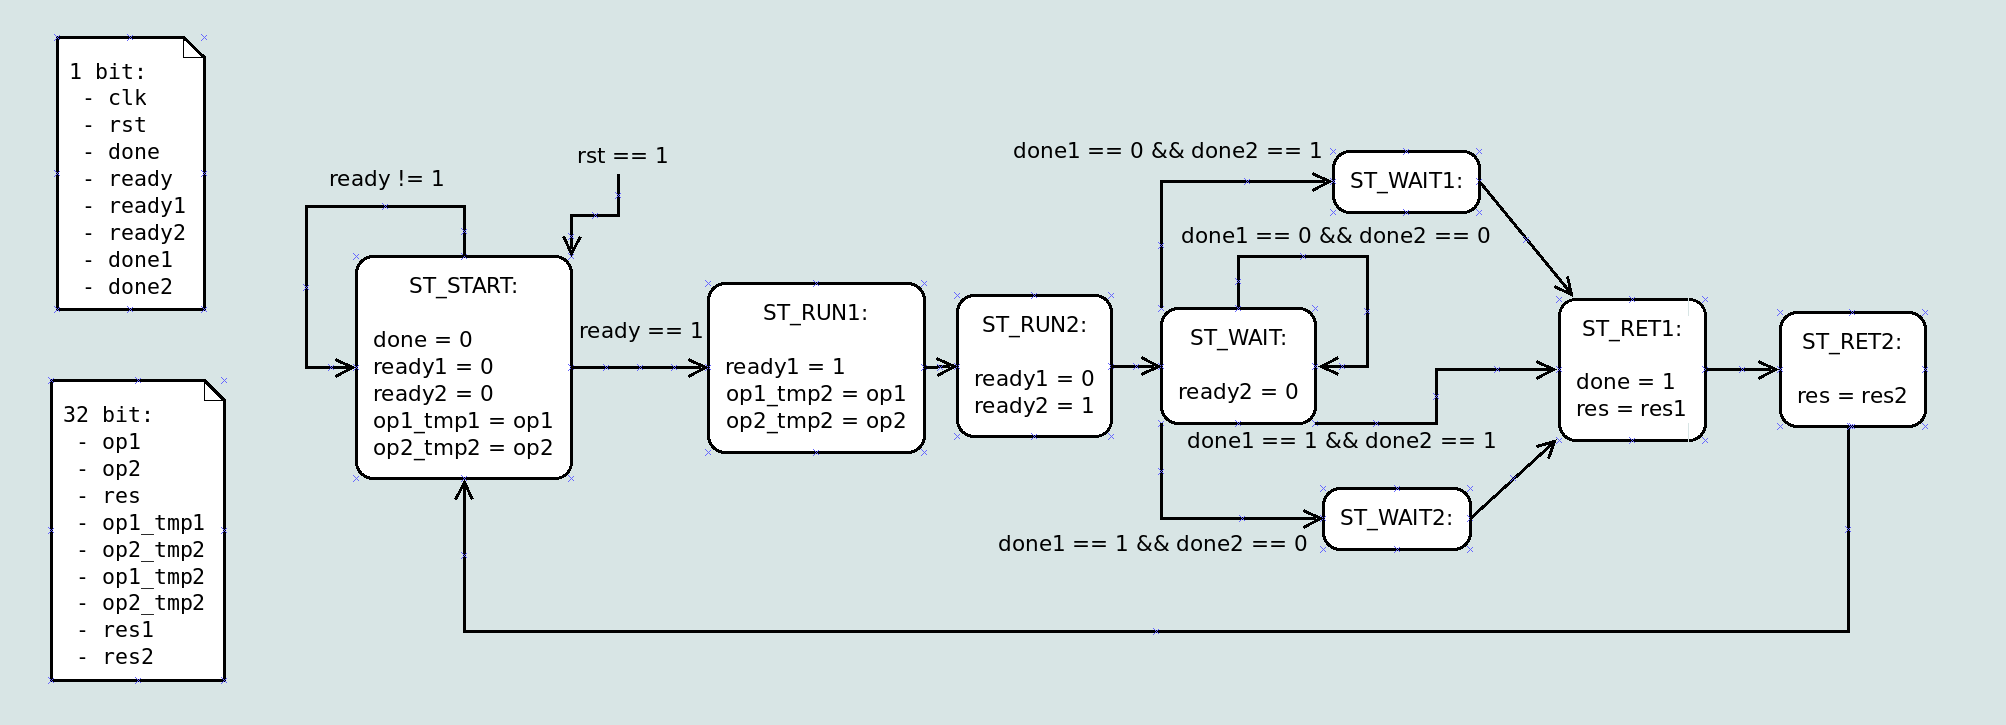
\includegraphics[width=\columnwidth]{figures/EFSM-top_level}
	\caption{Figura in formato piccolo, 2.}
	\label{fig:piccola2}
\end{figure}

\end{document}